%****************************************************************************
%*  Autor: Nicolas Peter Lane                                               *
%*  Data: 02/04/2015                                                        *
%*  Modelo LaTeX                                                            *
%*  sugest�es/d�vidas: lambdox@gmail.com                                    *
%*  									    *
%*  Licen�a GPL:              						    *
%*  Permission to use, copy, modify, and distribute this protocol and its   *
%*  documentation for any purpose, without fee, and without written         *
%*  agreement is hereby granted, provided that the above copyright notice,  *
%*  and the author appear in all copies of this protocol.                   *
%*                                                                          *
%****************************************************************************/

\documentclass[a4paper, ruledheader]{abnt}

\usepackage[brazilian]{babel} % Permite utilizar configuracoes da linguagem portugesa do Brasil e Inglesa
\usepackage[utf8]{inputenc} % Permite especificar codificacao das entradas (caracteres acentuados - � - sem usar \'a)
\usepackage{perl}
\usepackage{float}
\usepackage{psfrag}
\usepackage{subfig}
\usepackage{amsmath}%Permite usar f�rmulas matem�ticas
\usepackage{graphicx}
\usepackage{latexsym}
\usepackage{ragged2e} %Permite usar formata��o justificada /justify
\usepackage[Conny]{fncychap} 
\ChTitleAsIs

\begin{document}


\instituicao{Perl Brasil}
\autor{Heitor G., Nicolas P. Lane, Marcos F., Guilherme B., Pedro S., Marcos O., Gabriel M., Brian L., Felipe A., Junior O. 
}

\titulo{Apostila b\'asica de Perl}

\data{dezembro / 2015}


\capa

\setcounter{page}{1} % inicia a contagem do numero das paginas
\pagenumbering{roman} % define tipo de numeracao romana minuscula
% ====================================================================
% Contents
% ====================================================================
\tableofcontents


\setcounter{page}{0} % Reinicia a contagem do numero das paginas
\pagenumbering{arabic} % Numeracao dos capitulos arabica

\chapter{Introdu\c{c}\~ao}

Perl \'e uma linguagem de programa\c{c}\~ao de alto n\'ivel, usada em aplica\c{c}\~oes Web e Desktop. Ela foi desenvolvida por Larry Wall
em 1987, a sigla PERL significa ''\textit{Practical Extraction And Report Language}'' que traduzindo equivale a ''Linguagem Pr\'atica de Relat\'orio e 
Extra\c{c}\~ao''. Perl destaca-se por ser r\'apida, eficiente e de f\'acil manuten\c{c}\~ao. 

A comunidade Perl reuniu m\'odulos, classes, scripts e frameworks no CPAN (\textit{Comprehensive Perl Archive   Network}), reposit\'orio onde voc\^e pode 
encontrar quase tudo j\'a desenvolvido na linguagem. Perl também tornou-se muito popular fora do Brasil por ser uma linguagem que previne erros de 
seguran\c{c}a, sendo portanto muito pouco prov\'avel que voc\^e cometa algum erro de implementa\c{c}\~ao que comprometa a sua aplica\c{c}\~ao. 



\chapter{Ambiente de desenvolvimento}
 
\section{Interpretador perl} 
Usu\'arios de sistemas derivativos Unix, como Linux e BSD, possuem uma grande probablidade de que a sua distribui\c{c}\~ao/SO j\'a possua um interpretador 
Perl pr\'e-instalado. Aos usu\'arios Windows \'e necess\'ario instalar o ''\textit{Active Perl}'', que pode ser facilmente obtido em www.activestate.com. 
 
Caso sua distribui\c{c}\~ao por algum motivo n\~ao tiver o interpretador Perl pr\'e-instalado, \'e poss\'ivel instal\'a-lo usando algum dos comandos abaixo. 

\begin{itemize}
    \item{Ubuntu ou Debian: sudo apt-get install perl}
    \item{Arch Linux: Pacman S perl}
    \item{OpenSUSE: zypper install perl}
    \item{Fedora/Red Hat Enterprise: yum install perl}
\end{itemize}

\section{Editor de texto}  
\'E necess\'ario um editor de texto qualquer para escrever nossos c\'odigos, nessa apostila ser\'a usado o Sublime Text 3 
(dispon\'ivel via www.sublimetext.com/3) e o vim. 
\chapter{Hello World}
Vamos a escrita do primeiro programa em perl.  

\begin{figure}[!htb]
	\centering
	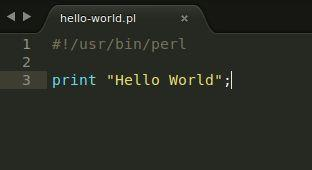
\includegraphics[width=0.3\textwidth]{../5_figuras/image1}
	\caption{Exemplo de implementa\c{c}\~ao}
\end{figure}

Na figura 1, a primeira linha ''\textit{\#!/usr/bin/perl}'', informa ao sistema que o c\'odigo passar\'a pelo interpretador perl, esta linha \'e 
necess\'aria para sistemas derivados do Unix, no Windows  o active perl configura uma instru\c{c}\~ao equivalente para o diret\'orio padr\~ao do sistema. 

Na 3$^a$ linha, o comando \textit{print} faz a escrita de dados para a sa\'ida padr\~ao de dados, neste caso, o monitor.  Sua sintaxe requer o uso de aspas duplas
por se tratar de um texto e o ponto e v\'irgula indica o fim de um comando.

Todo arquivo feito em Perl deve possuir a extens\~ao ''\textit{.pl}'', para executar um arquivo em Perl, deve-se abrir o promt ou o terminal e digitar o 
comando \textit{perl nomedoarquivo.pl} e pressionar Enter.
 
\chapter{Vari\'aveis}
O que \'e uma vari\'avel? Na programa\c{c}\~ao uma variável consiste de um bloco de mem\'oria capaz de armazenar e representar um valor ou express\~ao e este 
pode variar durante o decorrer da execu\c{c}\~ao do programa. Em Perl uma vari\'avel pode ser declarada como apresentado na figura 2. 

\begin{figure}[!htb]
	\centering
	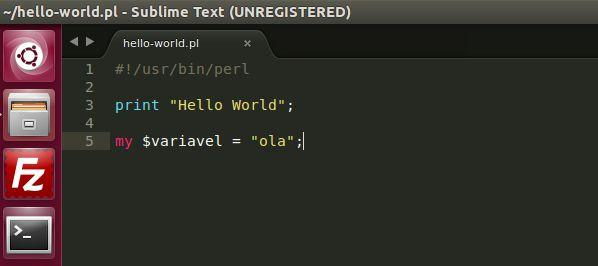
\includegraphics[width=0.5\textwidth]{../5_figuras/image2}
	\caption{Declarando-se uma vari\'avel}
\end{figure}

Toda vari\'avel possui um \$ antecedendo o seu nome, isto faz parte de sua sintaxe sendo portanto obrigat\'orio. O conte\'udo da vari\'avel \'e uma string, 
deste modo, tudo o que estiver dentro de aspas duplas ou simples \'e o conte\'udo da vari\'avel, finalizando com o ponto e v\'irgula como dito antes. Durante
a declara\c{c}\~ao da vari\'avel deve-se utilizar \textit{my} precedendo o seu nome, \textit{my \$nome\_da\_vari\'avel}.

Em Perl as vari\'aveis s\~ao dinamicamente tipadas, ou seja, n\~ao \'e necess\'ario definir o tipo de dado que aquela vari\'avel ir\'a suportar antes de 
seu uso. Segue um programa simples que realize a soma de alguns n\'umeros e escreva o seu resultado na tela.

\begin{figure}[!htb]
	\centering
	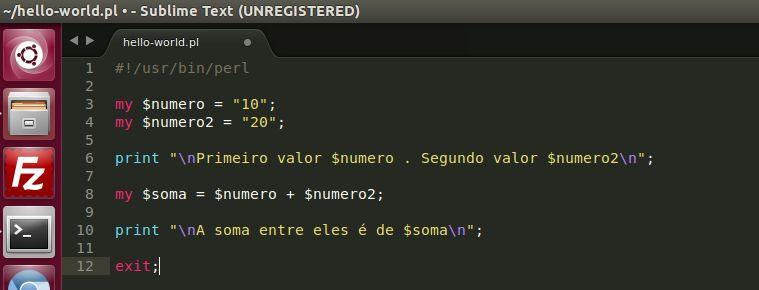
\includegraphics[width=0.5\textwidth]{../5_figuras/image3}
	\caption{Implementa\c{c}\~ao do algoritmo de soma}
\end{figure}

Na figura 3 pode-se ver que foi definido 2 vari\'aveis, \textit{\$numero = 10} e \textit{\$numero2 = 20}, logo depois \'e informado dados do usu\'ario, e 
na linha 8 \'e realizada a soma das 2 vari\'aveis que resulta no valor 30. O comando de escape ''\textit{\textbackslash n}'' indica uma quebra de linha, ele 
faz com que o conte\'udo que o procede seja escrito na pr\'oxima linha. Comandos de escape modificam a sa\'ida padr\~ao do programa. A sa\'ida do programa 
fica como apresentado na figura 4.

\begin{figure}[!htb]
	\centering
	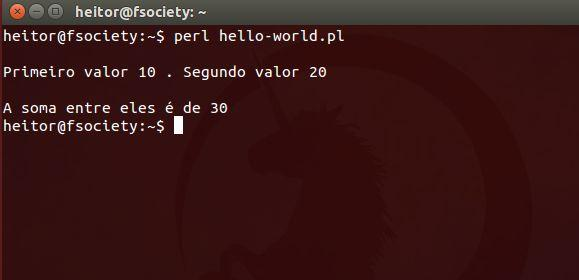
\includegraphics[width=0.4\textwidth]{../5_figuras/image4}
	\caption{Sa\'ida do algoritmo de soma}
\end{figure}

Uma lista adicional com os principais comandos de escape pode ser visto na figura 5.

\begin{figure}[!htb]
	\centering
	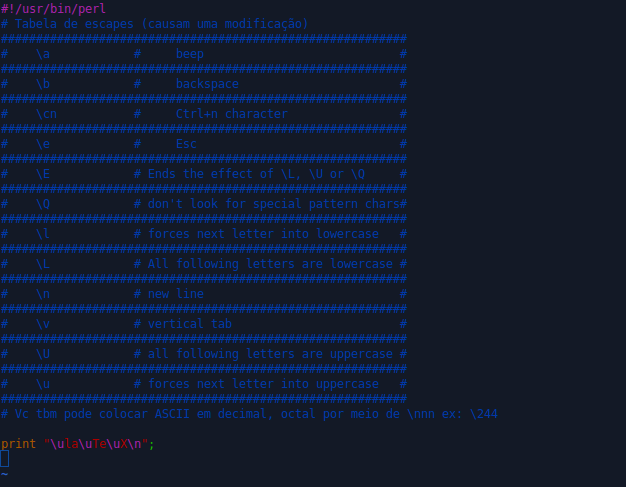
\includegraphics[width=0.45\textwidth]{../5_figuras/image5}
	\caption{Imagem 5: Trecho com principais comandos de escape}
\end{figure}


\chapter{Operadores}
Perl usa todos os mesmos operadores de C como apresentado na figura 6.

\begin{figure}[!htb]
	\centering
	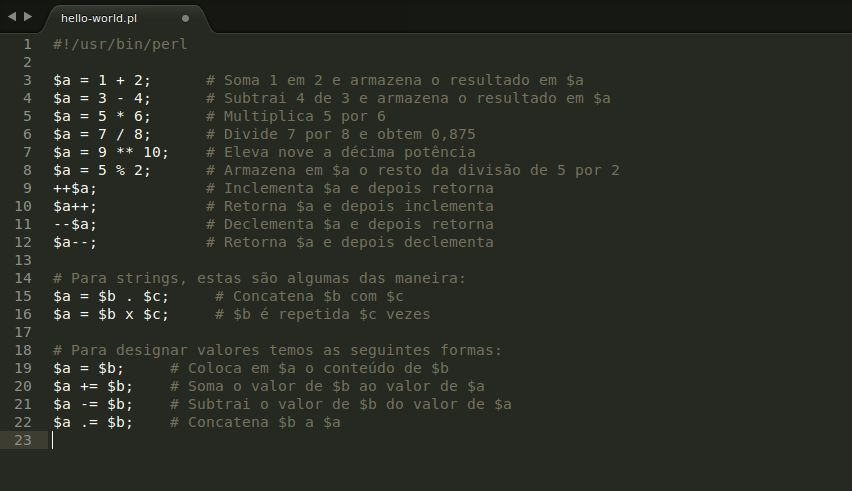
\includegraphics[width=0.8\textwidth]{../5_figuras/image6}
	\caption{Operadores}
\end{figure}


\chapter{Entrada de dados}

Agora ser\'a apresentado como capturar dados a partir da entrada padr\~ao e armazenar seu conte\'udo em uma vari\'avel.

\begin{figure}[!htb]
	\centering
	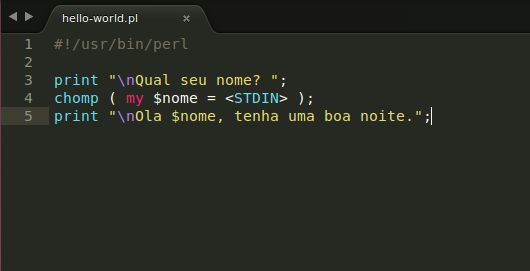
\includegraphics[width=0.5\textwidth]{../5_figuras/image7}
	\caption{Algoritmo com captura da entrada padr\~ao}
\end{figure}

Na figura 7, linha 4 a vari\'avel \$nome que recebe o valor de \textit{$<$STDIN$>$}, que \'e a fun\c{c}\~ao que l\^e uma linha da entrada padr\~ao, 
nesse caso, o teclado. O que \'e chomp? \'E a fun\c{c}\~ao que elimina o \'ultimo caractere caso esse \'ultimo caractere seja um o comando de escape 
respons\'avel pela quebra da linha (\textbackslash n). A sa\'ida do algoritmo segue na figura 8.

\begin{figure}[!htb]
	\centering
	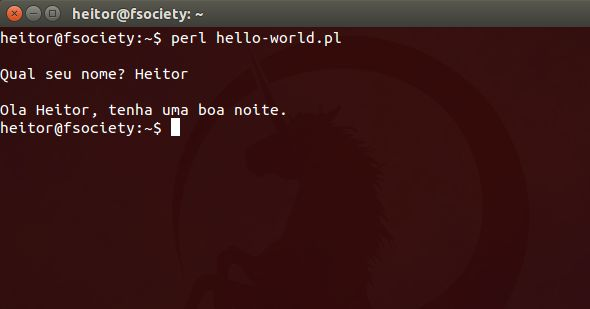
\includegraphics[width=0.5\textwidth]{../5_figuras/image8}
	\caption{Sa\'ida do algoritmo de captura da entrada padr\~ao}
\end{figure}

Hora de colocar o conhecimento adquirido em pr\'atica. 

\begin{figure}[!htb]
	\centering
	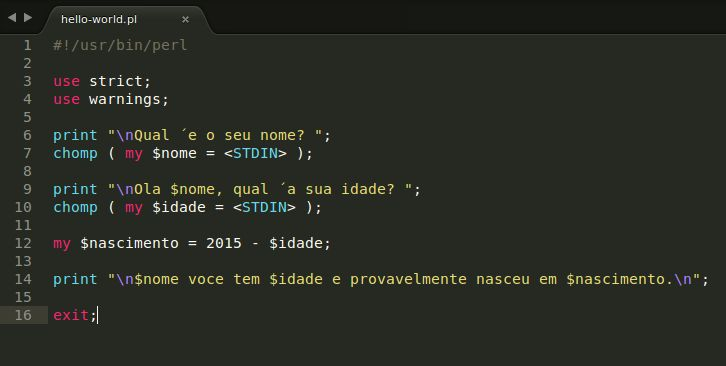
\includegraphics[width=0.5\textwidth]{../5_figuras/image9}
	\caption{Modelo de algoritmo a se adotar}
\end{figure}

Bom, a seguir \'e apresentado algumas alguns conceitos novos. O primeiro \'e o conceito de m\'odulos; m\'odulos s\~ao bibliotecas que mudam o modo de 
interpreta\c{c}\~ao do Perl. Na figura 9, na 3$^a$ e 4$^a$ linha s\~ao usados os m\'odulos \textit{strict} e \textit{warnings}. O \textit{use} 
indica ao interpretador quais m\'odulos a serem ativados.

\textit{strict} e \textit{warnings} ajuda a evitar os principais erros e enganos comuns nos c\'odigos em perl, por isso s\~ao extremamente \'uteis e 
recomenda-se o seu uso. 
  
Na linha 12 \'e efetuada uma opera\c{c}\~ao m\'atematica simples para descobrir o ano de nascimento do usu\'ario a partir na idade informada, a l\'ogica
para resolver esse problema \'e basicamente a idade menos o ano informado que retornar\'a o ano de nascimento. Depois \'e feita uma chamada de \textit{print}
para escrita na sa\'ida padr\~ao de dados. A sa\'ida \'e apresentada na figura 10.

\begin{figure}[!htb]
	\centering
	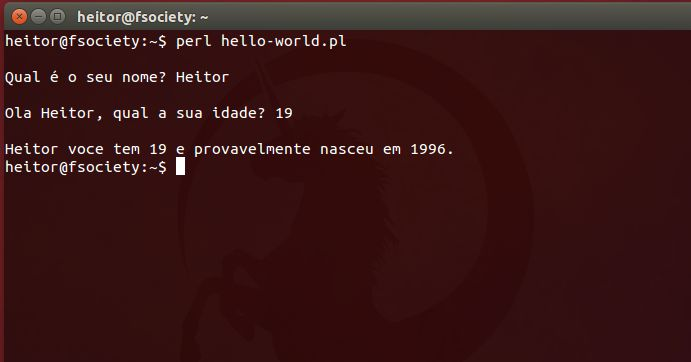
\includegraphics[width=0.5\textwidth]{../5_figuras/image10}
	\caption{Sa\'ida do algoritmo}
\end{figure}
\chapter{Tomando decis\~oes}

Um c\'odigo pode ter rotinas para a resolu\c{c}\~ao de um determinado problema necessitem serem seguidos, enquanto outros n\~ao o sejam. 
Rotinas s\~ao sequ\^encias de linhas de c\'odigo. A cria\c{c}\~ao de uma estrutura de decis\~ao permite controlar quais rotinas devem ser executadas em 
detrimento de outras. Para este fim o Perl possui fun\c{c}\~oes de compara\c{c}\~ao (\textit{if, else} e \textit{elsif}). \textit{if} traduzido para o 
portugu\^es fica ''se''. Um exemplo de seu funcionamento \'e apresentado na figura 11.   

\begin{figure}[!htb]
	\centering
	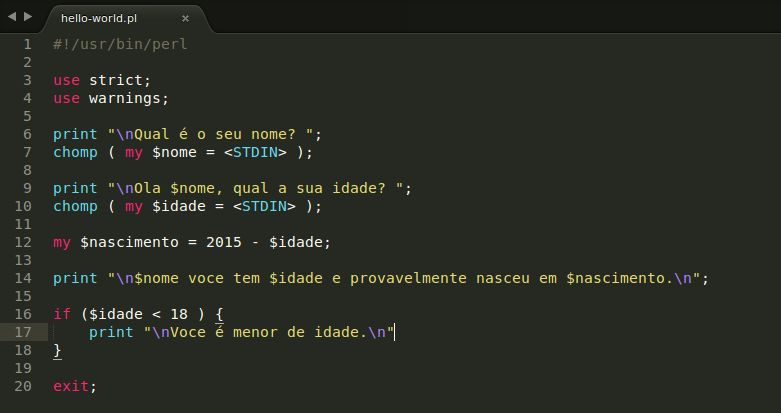
\includegraphics[width=0.7\textwidth]{../5_figuras/image11}
	\caption{Algoritmo com estrutura de decis\~ao}
\end{figure}

Na figura 11, linha 16 pode-se ver o que o \textit{if} compara se a vari\'avel que cont\'em a idade informada pelo usu\'ario \'e menor que 18, caso a idade 
seja menor, \'e requisitado que um trecho de c\'odigo respons\'avel por imprimir a mensagem ''Voc\^e \'e menor de idade'' para a sa\'ida padr\~ao seja chamada.

A sa\'ida \'e apresentada na figura 12.

\begin{figure}[!htb]
	\centering
	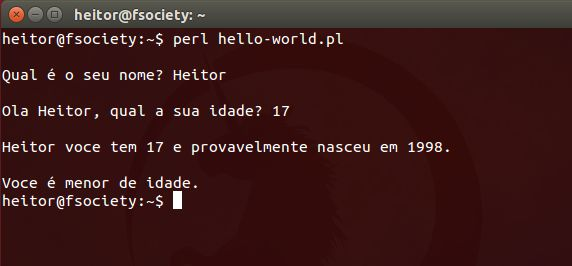
\includegraphics[width=0.7\textwidth]{../5_figuras/image12}
	\caption{Sa\'ida do algoritmo com estrutura de decis\~ao}
\end{figure}

Com o \textit{if} pode-se comparar tanto valores num\'ericos quanto cadeias de caracteres (\textit{strings}). O \textit{else} pode ser traduzido como 
''sen\~ao'', seu uso em conjunto com o if \'e caracteriza uma estrutura de decis\~ao composta, seu funcionamento pode ser visto na figura 13.

\begin{figure}[!htb]
	\centering
	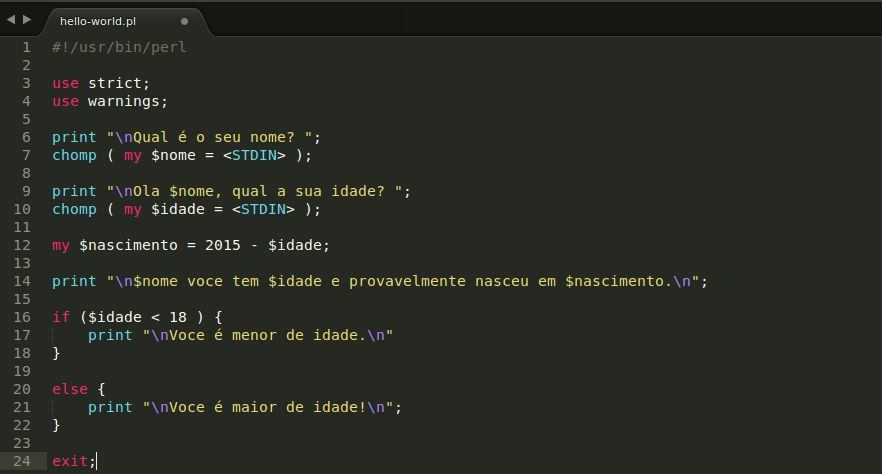
\includegraphics[width=0.7\textwidth]{../5_figuras/image13}
	\caption{Algoritmo com estrutura de decis\~ao composta}
\end{figure}

\clearpage 

Logicamente se a idade do usu\'ario n\~ao for menor que 18, ent\~ao ele ser\'a  maior de idade, como apresentado na figura 14.

\begin{figure}[!htb]
	\centering
	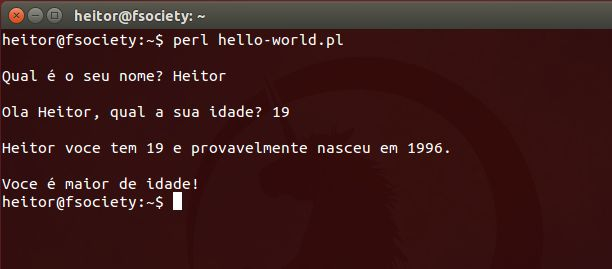
\includegraphics[width=0.5\textwidth]{../5_figuras/image14}
	\caption{Sa\'ida do algoritmo com estrutura de decis\~ao composta}
\end{figure}

E finalmente, o \textit{elsif}, sua tradu\c{c}\~ao \'e equivalente a ''sen\~ao se''. O uso conjuto de \textit{if}, \textit{elsif} e \textit{else} permite uma
estrutura de decis\~ao muito mais abrangente e precisa, chamada de estrutura de decis\~ao completa, como apresentado na figura 15.

\begin{figure}[!htb]
	\centering
	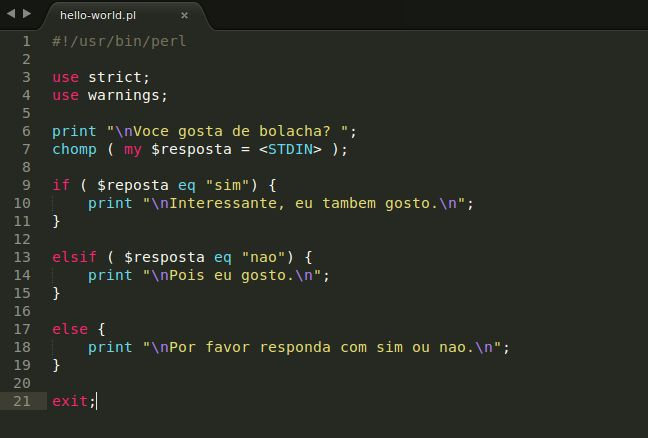
\includegraphics[width=0.6\textwidth]{../5_figuras/image15}
	\caption{Algoritmo com estrutura de decis\~ao completa}
\end{figure}

Na figura 16, linha 9 observa-se que a resposta dada foi  ''sim'', j\'a na linha 13 observa-se outro caso onde a resposta dada foi ''n\~ao'', caso 
a resposta dada n\~ao fosse igual a nenhum dos casos abordados nas condi\c{c}\~oes anteriores da estrutura de decis\~ao o \textit{else} pede para responder 
corretamente. 

\begin{figure}[!htb]
	\centering
	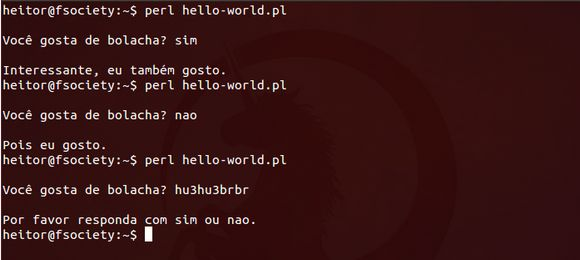
\includegraphics[width=0.4\textwidth]{../5_figuras/image16}
	\caption{Sa\'ida do algoritmo com estrutura de decis\~ao completa}
\end{figure}





\chapter{Entrada de dados}

O Perl possui dois conjuntos de operadores de compara\c{c}\~ao. 

\begin{figure}[!htb]
	\centering
	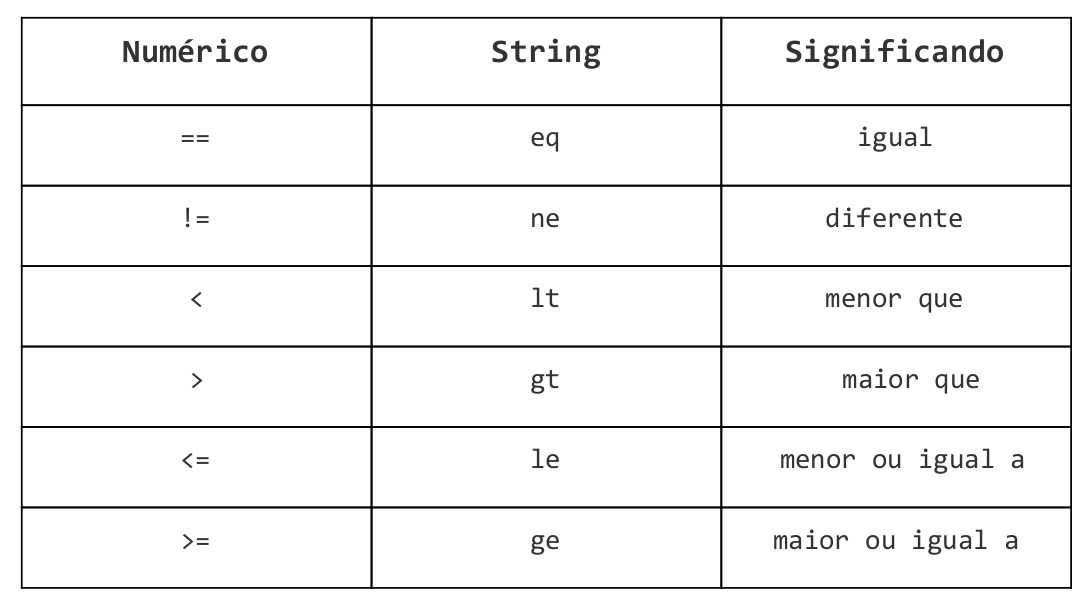
\includegraphics[width=0.5\textwidth]{../5_figuras/image17}
	\caption{Tabela com operadores de compara\c{c}\~ao}
\end{figure}



\chapter{Laços de repeti\c{c}\~ao}

Em Perl quando certa instru\c{c}\~ao precisa ser repetida uma certa quantidade, deve-se fazer uso de um comando de estrutura de repeti\c{c}\~ao, o comando 
\textit{while} \'e um exemplo, \textit{while} significa, ''enquanto''. Vamos usar como base o exemplo na figura 18.

\begin{figure}[!htb]
	\centering
	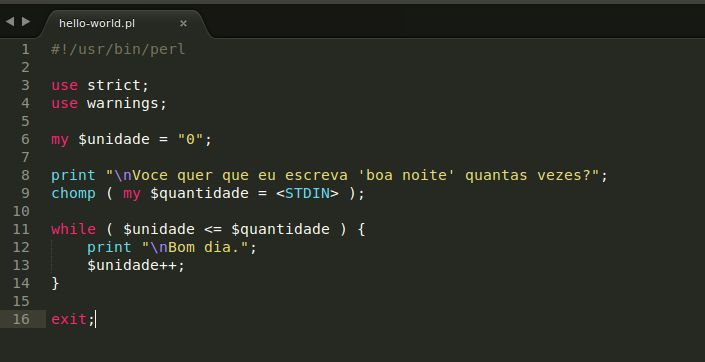
\includegraphics[width=0.5\textwidth]{../5_figuras/image18}
	\caption{Algoritmo com estrutura de repeti\c{c}\~ao while}
\end{figure}

Na 6$^a$ linha definida a vari\'avel \textit{\$unidade = 0}, logo depois, \'e requisitado ao usu\'ario que informe uma quantidade n\'umerica de seu gosto, 
ent\~ao na 11$^a$ linha \'e desenvolvida a seguinte l\'ogica; enquanto \textit{\$unidade $<$= \$quantidade} ser\'a escrito \textit{bom dia} na tela para 
ent\~ao retornar o valor da vari\'avel \$unidade, incrementando-o posteriormente.

\begin{figure}[!htb]
	\centering
	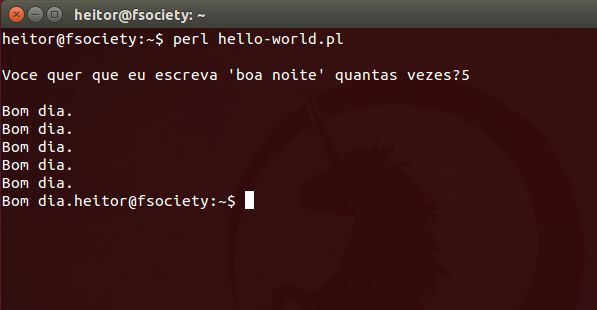
\includegraphics[width=0.5\textwidth]{../5_figuras/image19}
	\caption{Sa\'ida do algoritmo com estrutura de repeti\c{c}\~ao while}
\end{figure}

Outro operador para o mesmo fim \'e o \textit{for}, como \'e apresentado na figura 20.

\begin{figure}[!htb]
	\centering
	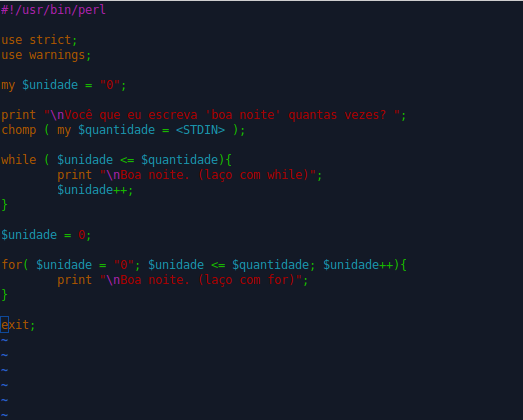
\includegraphics[width=0.5\textwidth]{../5_figuras/image20}
	\caption{Algoritmo com estrutura de repeti\c{c}\~ao for}
\end{figure}

O \textit{while} e o \textit{for} possuem praticamente a mesma finalidade, mas voc\^e deve saber quando usar cada um deles. A sa\'ida desses dois casos 
ser\~ao exatamente iguais.

Que tal deixarmos nossos programas um tanto mais coloridos? Para isso ser\'a usado o m\'odulo \textit{Term::ANSIColor}. Caso sejas um usu\'ario Windows, use 
o m\'odulo \textit{Win32::Console::ANSI}.

H\'a uma grande chance de que sua distribui\c{c}\~ao/SO n\~ao tenha este m\'odulo pr\'e-instalado, para instal\'-lo digite o comando a seguir no terminal 
\textit{cpan install Term::ANSIColor} ou no prompt \textit{cpan install Win32::Console::ANSI} respectivamente. A instala\c{c}\~ao de qualquer modulo segue o 
mesmo padr\~ao, o comando \textit{cpan} chama o mesmo avisando que deve ser instalado o m\'odulo \textit{Term::ANSIColor}. Uma vez conclu\'ida a 
instala\c{c}\~ao, vamos a a\c{c}\~ao!

\begin{figure}[!htb]
	\centering
	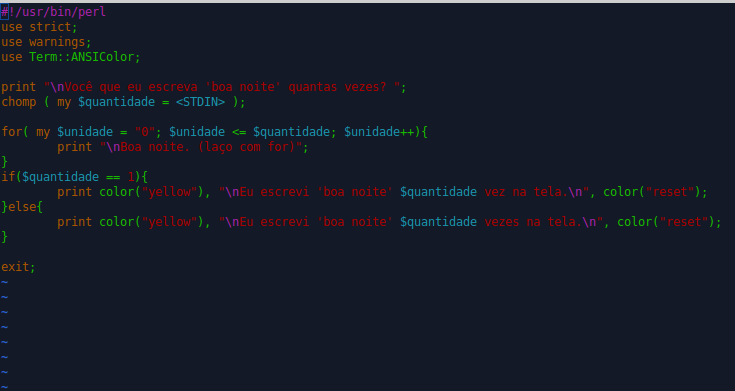
\includegraphics[width=0.5\textwidth]{../5_figuras/image21}
	\caption{Algoritmo com m\'odulo para alterar a cor do texto da sa\'ida padr\~ao do programa}
\end{figure}

Este m\'odulo n\~ao necessita de muita explica\c{c}\~ao, na figura 21, 5$^a$ linha o m\'odulo \'e requisitado e ativado, na sequ\^encia, ocorre uma o envio de
dados para a sa\'ida padr\~ao com a cor que desejes, essa funcionalidade \'e realizada dentro do comando \textit{print}, colocando a cor desejada com a 
seguinte express\~ao \textit{color(''nome'')}. Os nomes das cores devem ser escritos em ingl\^es ingl\^es, ao final do \textit{print} deve-se usar a 
instru\c{c}\~ao de altera\c{c}\~ao das cores com \textit{reset} para retorn\'a-las ao seu estado inicial, como apresentado na figura 22.  

\begin{figure}[!htb]
	\centering
	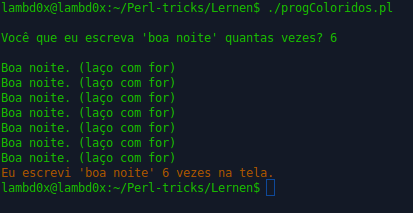
\includegraphics[width=0.4\textwidth]{../5_figuras/image22}
	\caption{Sa\'ida do algoritmo}
\end{figure}


\chapter{Manipula\c{c}\~ao de arquivos e comandos no sistema}
Manipular arquivos e executar comandos no sistema \'e muito simples em Perl, pode-se criar, editar e excluir arquivos de texto e muitas outras coisas 
interessantes. No exemplo da figura 23 pode-se observar que foi feito o uso do comando \textit{system (''comando do sistema'');}. O comando \textit{system} 
\'e respons\'avel por avisar que o conte\'udo entre parenteses e aspas ser\'a executado diretamente no sistema, sendo assim, os comandos podem variar de SO 
para SO. O comando \textit{mkdir} \'e um comando do sistema Linux que \'e respons\'avel por criar diret\'orios.

\begin{figure}[!htb]
	\centering
	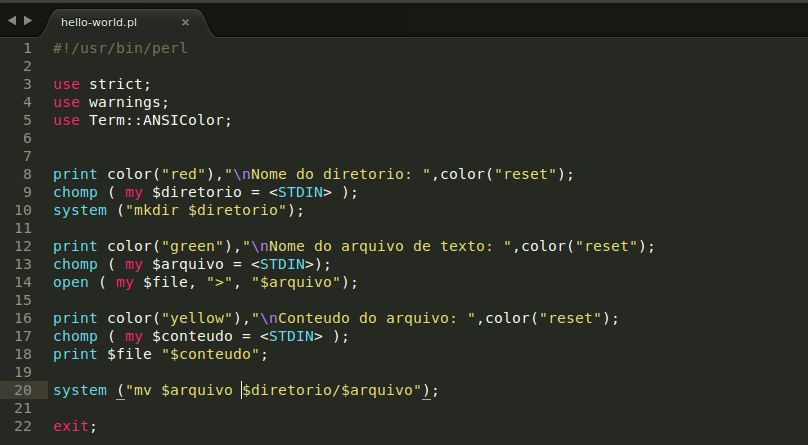
\includegraphics[width=0.5\textwidth]{../5_figuras/image23}
	\caption{Algoritmo executando tarefas no sistema}
\end{figure}

\clearpage

Observa-se o pedido para que o usu\'ario fornecesse o nome do diret\'orio para posteriormente este ser criado, na sequ\^encia \'e requisitado o nome do 
arquivo, sedno criado caso este j\'a n\~ao exista e finalmente \'e requisitado a escrita de conte\'udo deseja que exista no arquivo. J\'a na 20$^a$ linha, 
o arquivo \'e movido para o diret\'orio criado no in\'icio do nosso c\'odigo, um exemplo de sa\'ida pode ser visto na figura 24.

\begin{figure}[!htb]
	\centering
	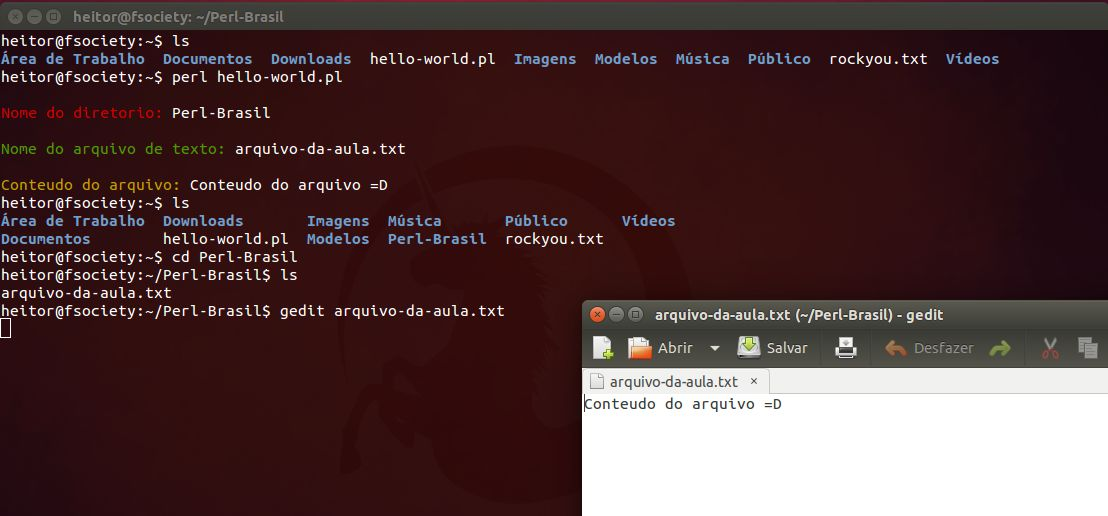
\includegraphics[width=0.8\textwidth]{../5_figuras/image24}
	\caption{Sa\'ida do algoritmo executando tarefas no sistema}
\end{figure}

\begin{itemize}
    \item{\$arquivo: abre ARQUIVO apenas para leitura (o mesmo que \textit{$<$\$arquivo);}}
    \item{\textit{$>$\$arquivo}: abre ARQUIVO para escrita, criando-o caso ainda n\~ao exista}
    \item{\textit{$>>$\$arquivo}: abre ARQUIVO para modificação (append)} 
    \item{\textit{+$>$\$arquivo}: abre ARQUIVO para leitura/escrita. }
\end{itemize}


 
\chapter{Considera\c{c}\~oes finais}

Infelizmente chegamos ao final desta apostila, mais cont\'udo pode ser adicionado por qualquer pessoa que deseje contribuir com o projeto. As apostilas de n\'ivel
intermedi\'ario e avan\c{c}ado necessita de mais pessoas colaborando com o projeto para que sua vers\~ao revisada seja entregue. 

A quem leu at\'e o fim, fica o convite para que acompanhem e fa\c{c}am parte da comunidade Perl Brasil nas redes sociais.
\begin{itemize}
    \item{https://fb.com/groups/PerlBrasilOficial}
    \item{https://fb.com/PerlBrOficial} 
    \item{https://github.com/HeitorG/PerlBrasil}
    \item{https://twitter.com/Perl\_Brasil}
\end{itemize}

\begin{figure}[!htb]
	\centering
	
\includegraphics[width=0.9\textwidth]{../5_figuras/image29}
\end{figure}

\section{Ci\^encia Hacker} 
\begin{itemize}
    \item{S\'itio: www.cienciahacker.com.br} 
    \item{Github: www.github.com/cienciahacker/index}
    \item{Facebook: www.fb.com/CienciaHacker}
    \item{Grupo: fb.com/groups/cienciahacker}
    \item{Twitter: twitter.com/cienciahacker}
    \item{YouTube: www.youtube.com/user/cienciahacker}
    \item{Vimeo: www. twitter.com/cienciahacker}
    \item{IRC: www.cienciahacker.com.br/irc} 
\end{itemize}

\section{WebSchool}
\begin{itemize}
    \item{S\'itio: www.webschool.io}
    \item{Github: www.github.com/Webschoolio} 
    \item{Facebook: www.fb.com/webschool.io}
    \item{Youtube: http://www.youtube.com/channel/UCKdo1RaF8gzfhvkOdZv\_ojg} 
\end{itemize}

\section{Contato}
\noindent
Heitor G. cold@protonmail.com 				\\
Nicolas P. Lane https://github.com/lambd0x		\\
Marcos F. github.com/marcosflorencio	 		\\
Guilherme B. github.com/guuibayer			\\
Pedro S. github.com/PedroSouza				\\
Marcos O. github.com/methz				\\
Gabriel M. fb.com/gabriel.dutra.47884754		\\
Brian L. fb.com/profile.php?id=100010099237181		\\
Felipe A. fb.com/fofinhocauai				\\
Junior O. fb.com/EuuulSexy				\\ 



 
\end{document}
